\def\QRCODE{TB_IPR_TUT.IMG.pixel_topological_description_pythonqrcode.png}
\def\QRPAGE{http://www.iptutorials.science/tree/master/TB_IPR/TUT.IMG.pixel_topological_description/python}
\pcorrectionsection{Python correction}


\subsection{Toplogical description}
The operations are not difficult, except that the $CAdj_4$ should be coded carefully.

\begin{python}
def nc(A):
    # A : block 3x3, binary
    # complementary set of A
    invA=1-A;
    # neighborhoods
    V8=np.ones((3,3)).astype(int);
    V8_star=np.copy(V8);
    V8_star[1,1] = 0;
    V4=np.array([[0, 1, 0],[1, 1, 1],[0, 1, 0]]).astype(int);
    # intersection is done by the min operation
    X1=np.minimum(V8_star,A);
    TT8=np.sum(X1);
    L, T8 = mes.label(X1, structure=V8);
    # The C-ajd-4 might introduce some problems if a pixel is not 4-connected
    # to the central pixel
    X2=np.minimum(V8,invA);
    Y=np.minimum(X2,V4);
    X=morpho.reconstruction(Y,X2,selem=V4);
    L, T8c = mes.label(X, structure=V4);
    
    return T8, T8c, TT8
\end{python}

\begin{figure}[htbp]
\centering
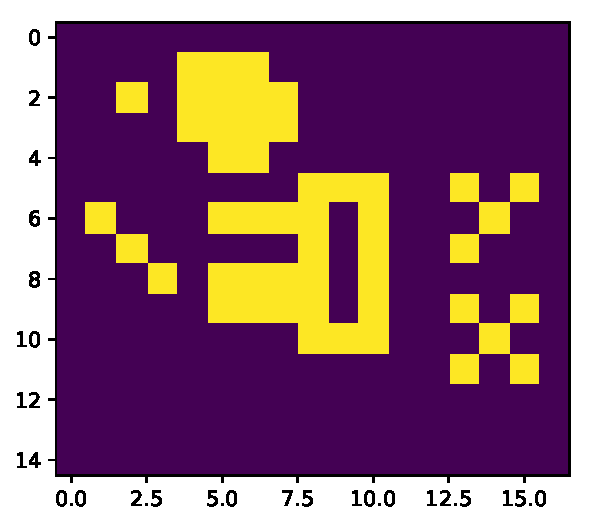
\includegraphics[width=.4\textwidth]{original.pdf}\hspace{15mm}
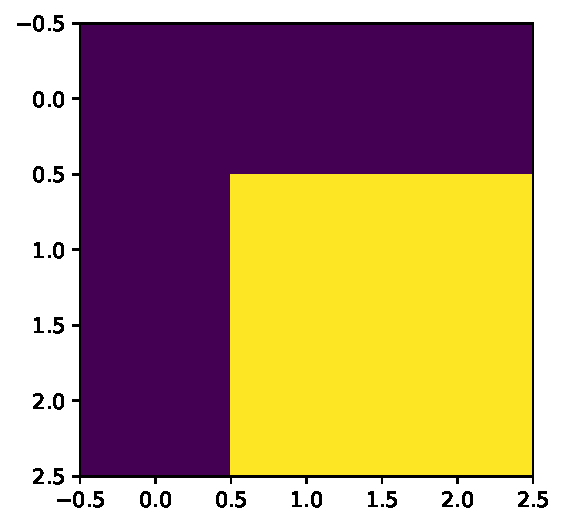
\includegraphics[width=.3\textwidth]{window.pdf}
\caption{Extraction of the window centered in $x=(1,4)$, given as (row,col).}
\label{fig:topological_description:python:example}
\end{figure}

\subsection{Topological classification}
The different types are given by the following code.
\begin{python}
def nc_type(X):
    # evaluates the connectivity numbers
    a,b,c=nc(X);
    if (a==0):
        y=1; # isolated point
    if ((a==1) and (b==1) and (c>1)): 
        y=5;  # border point
    if (b==0):
        y=7;  # interior point
    if ((a==1) and (b==1) and (c==1)):
        y=6;  # end point
    if (a==2):
        y=2;  # 2-junction point
    if (a==3):
        y=3;  # 3-junction point
    if (a==4):
        y=4;  # 4-junction point:
    return y; 
\end{python}
In order to perform the classification of all pixels of an image, one has to loop over all the pixels, except the ones at the sides. The results are presented in Fig.\ref{fig:topological_description:python:classification}

\begin{python}
def classification(A):
     # for the whole image
    m, n = A.shape
    B=np.zeros((m,n));
    for i in range(1, m-1):
        for j in range(1, n-1):
            if A[i,j]> 0:
                X=A[i-1:i+2,j-1:j+2];
                B[i,j]=nc_type(X);
    return B
\end{python}

\begin{figure}[htbp]
\centering
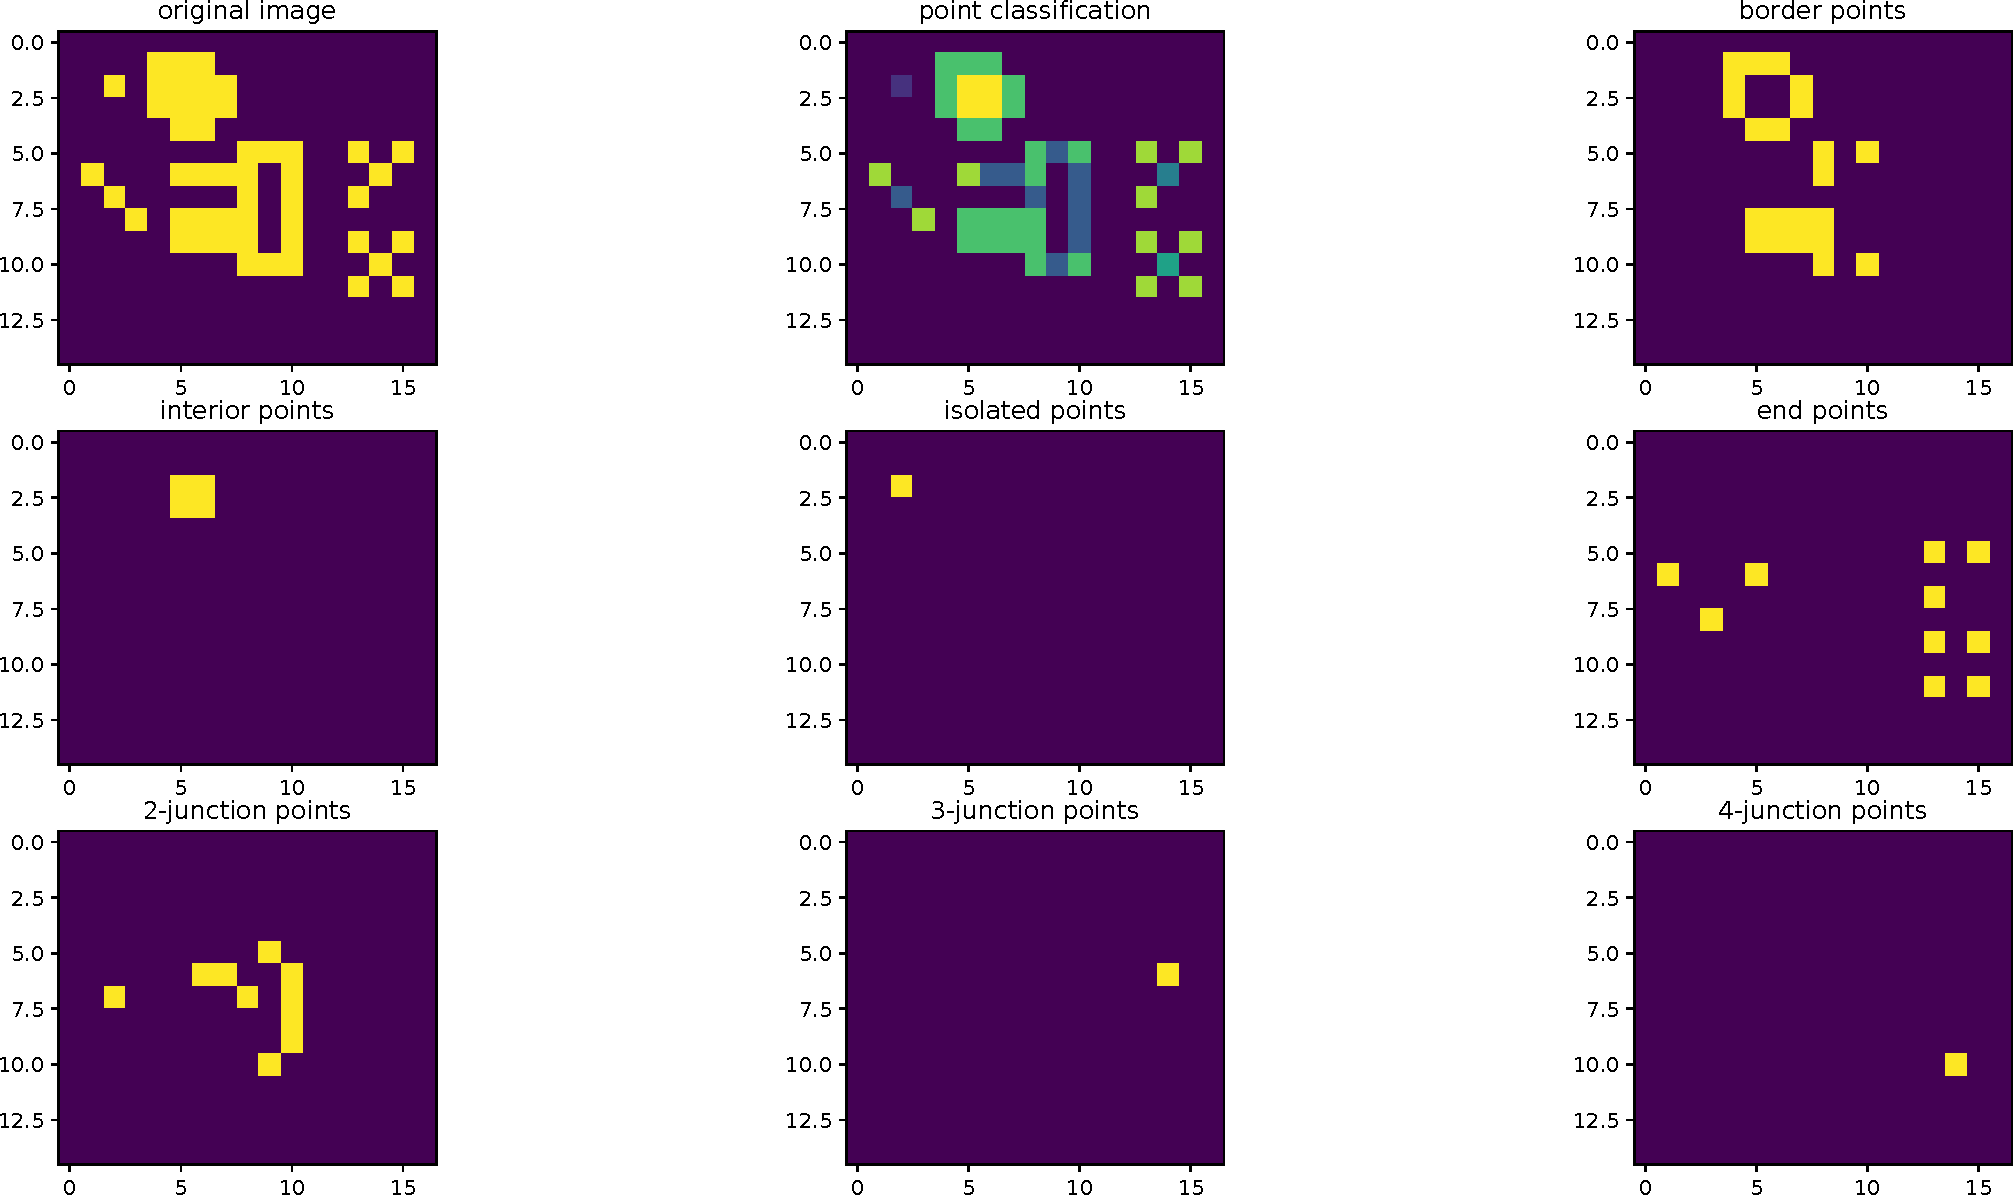
\includegraphics[width=\textwidth]{classif.pdf}
\caption{Classification of all the pixels of the the original image.}
\label{fig:topological_description:python:classification}
\end{figure}
